%!TEX root = ../main.tex

\section{Design} % (fold)
\label{sec:design}

Now that the list of requirements have been created, it is time to create a plan of how the product is going to fulfill these requirements. 
When that has been done the weather categories has to be delimited into a realistic amount of weather conditions. 
After that the visual and audial elements have to be found by pre-testing. 
In the end when the sounds and pictures have been found it is time to create the blueprint of how the pictures should look like and how the sounds is going to be created.

\begin{figure}[!htbp]
    \centering
    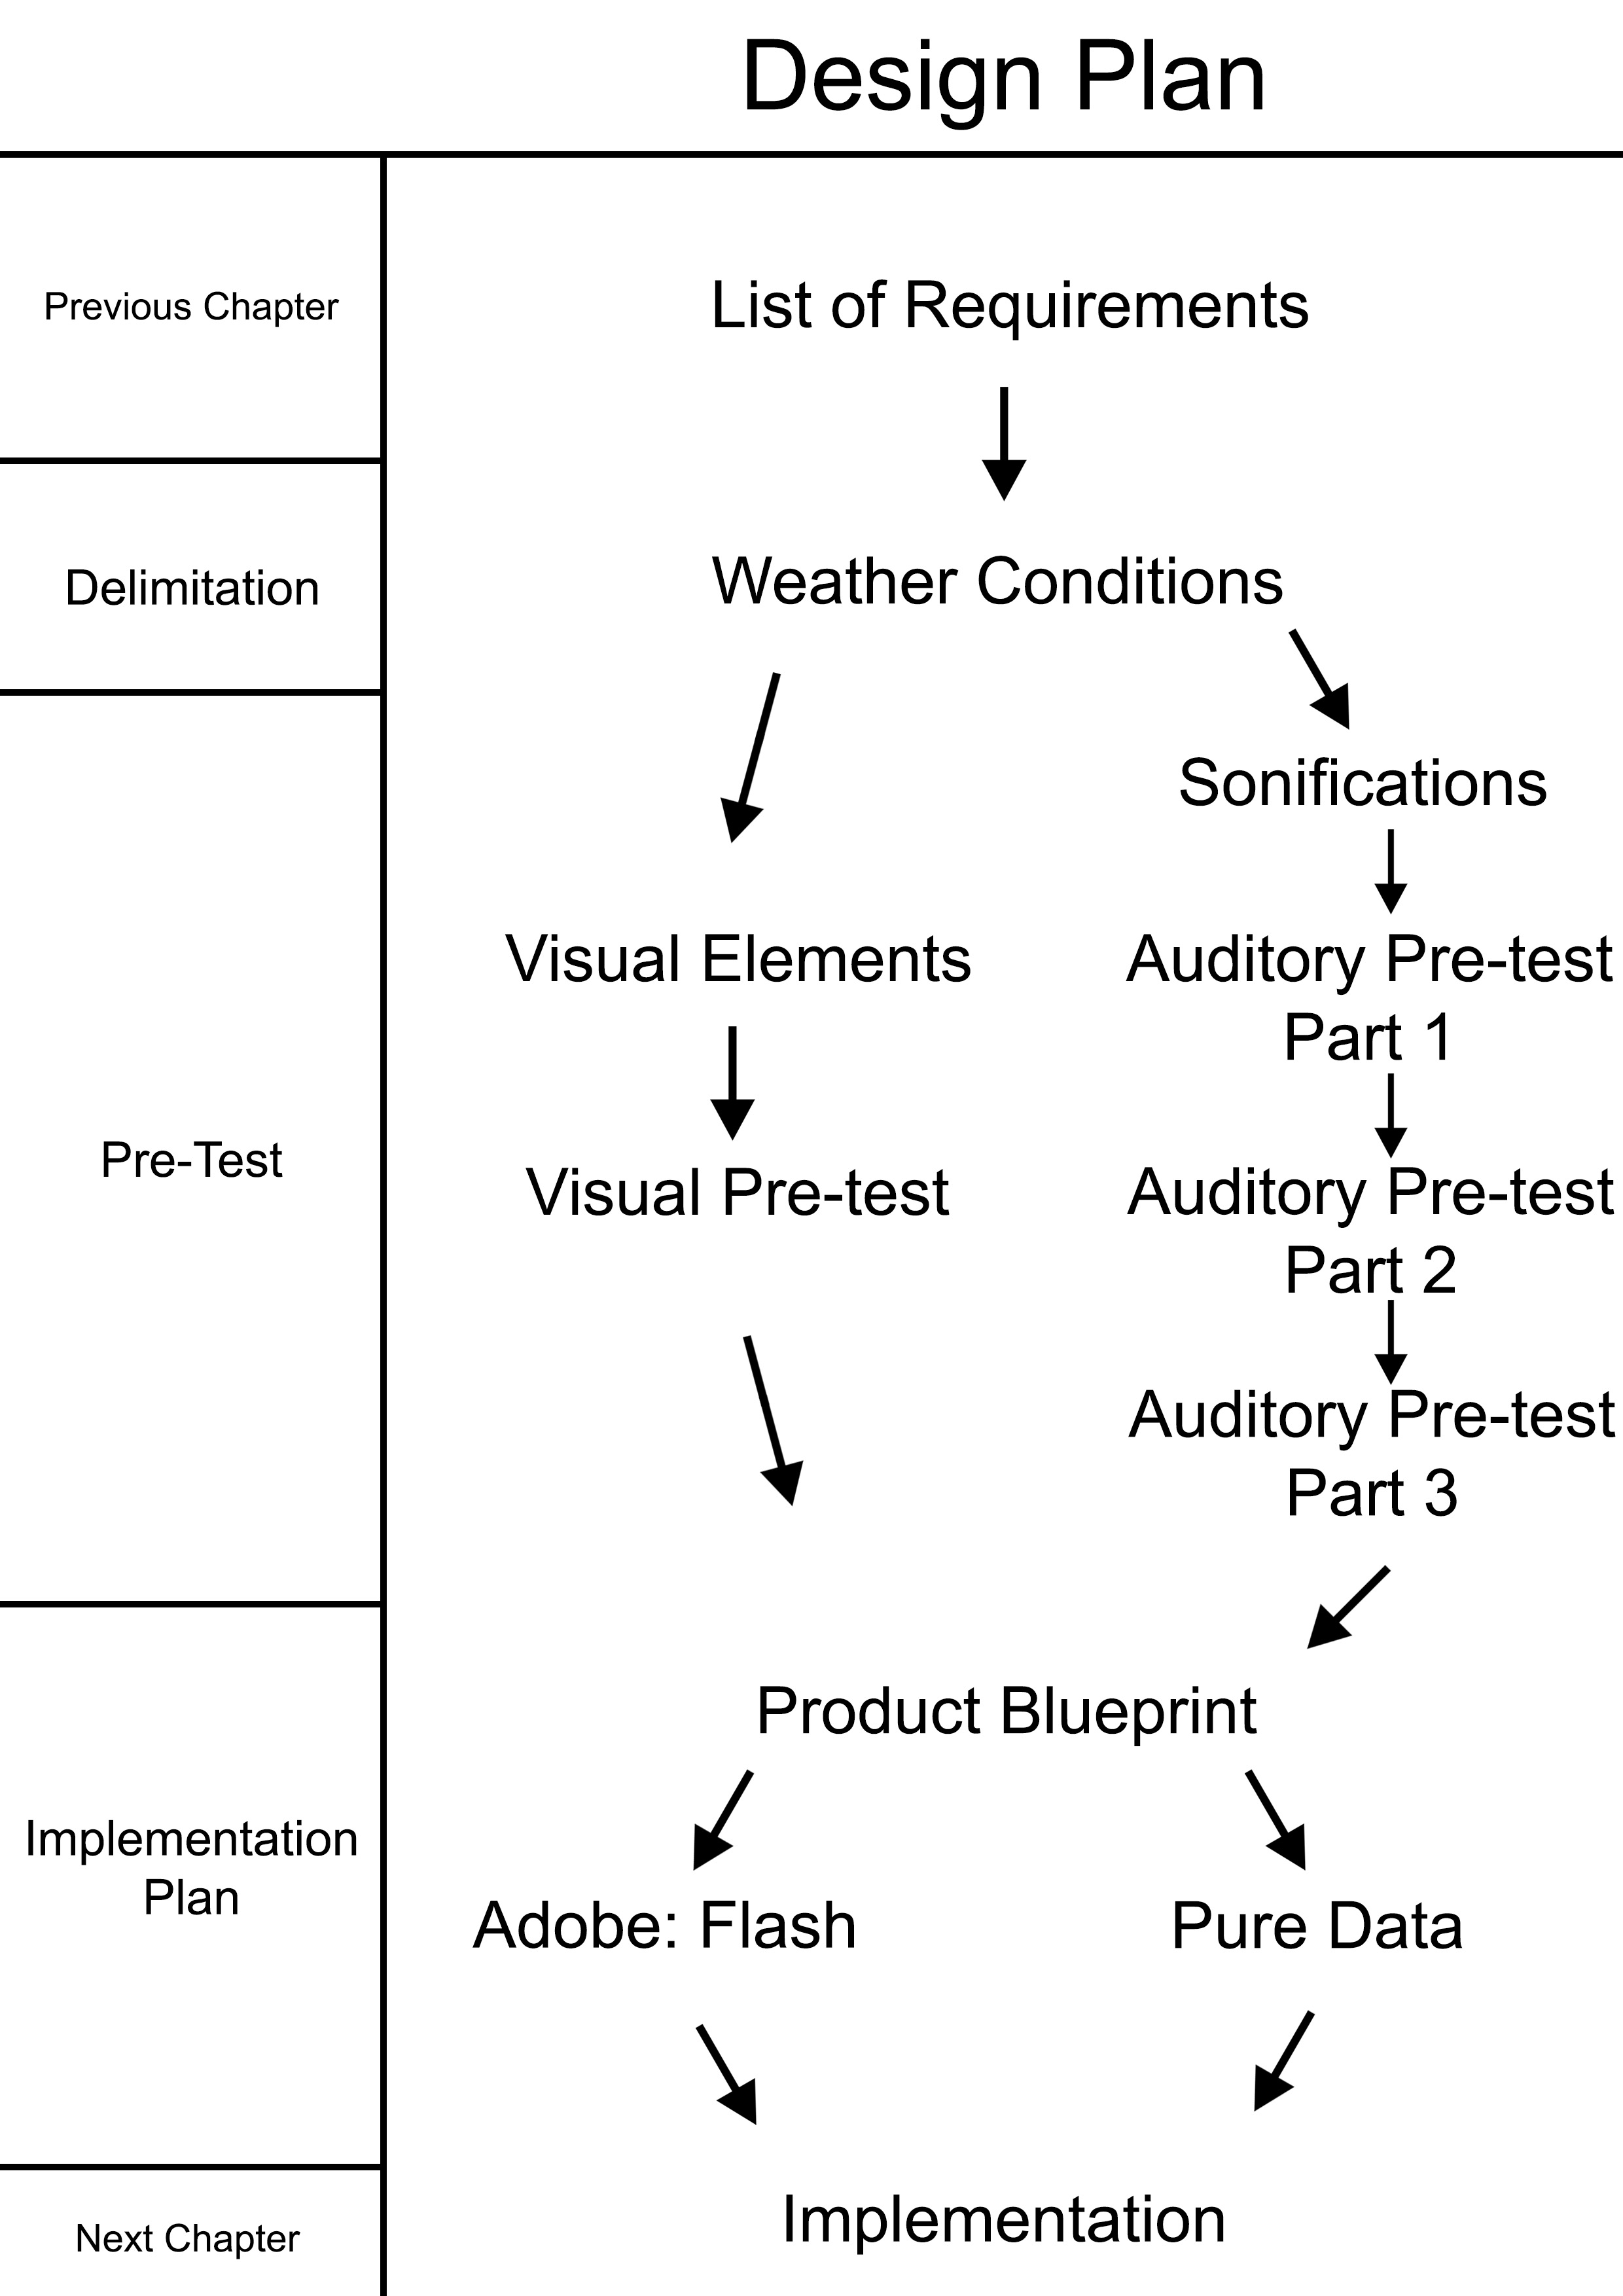
\includegraphics[width=.5\textwidth]{images/Design1.jpg}
    \caption{Plan for design process}
    \label{fig:design1}
\end{figure}


\subsection*{A design to meet all the requirements} % (fold)
\label{sub:a_design_to_meet_all_the_requirements}



% subsection a_design_to_meet_all_the_requirements (end)


\subsection*{Weather Conditions} % (fold)
\label{sub:weather_conditions}

There are a lot of different kinds of weather data. 
Since it is not possible to cover every single category of weather data within the projects time limit, we made the decision to make a delimitation of the categories.


Based on the research from the weather applications the following raw weather data list was created.

\subsubsection*{Raw list of weather data} % (fold)
\label{ssub:raw_list_of_weather_data}

\begin{itemize}
     \item \textbf{Temperature/Dewpoint} - Current air temperature 2 meters above terrain.
     \item \textbf{Wind speed} - Average wind speed over 10 minutes, 10 meters above terrain.
     \item \textbf{Wind direction} - Average wind direction in degrees.
     \item \textbf{Air pressure} - Pressure at sea level measured i hPa (Hectopascal).
     \item \textbf{Humidity} - Current relative humidity measured 2 meters above terrain, measured in percent.
     \item \textbf{Precipitation} - Rain/sleet/snow/hail over the past ten minutes measured in mm.
     \item \textbf{Sun hours} - Hours with sun in a day.
     \item \textbf{Pollen Forecast} - The potency of the pollen. 
     \item \textbf{Sunrise / sunset} - Time of day where the sun rises and sets.
     \item \textbf{Cloud cover}
     \item \textbf{Wind chill} - The winds effect on air temperature.
     \item \textbf{Visibility} - How far can you see with clear line of sight.
     \item \textbf{UV-index} - Intensity of UV radiation.
     \item \textbf{Fronts} 
     \item \textbf{Source Regions} - Where the air is coming from.
     \item \textbf{Drought} - Risk of drought. Presented as a scale.
 \end{itemize}

After going through the data on the raw list we found that many of the weather categories didn’t suit into our project. 
So we decided to only taking relevant weather data that people normally would use in an everyday situation.

% subsubsection raw_list_of_weather_data (end)


\subsubsection*{List of relevant data} % (fold)
\label{ssub:list_of_relevant_data}

\begin{itemize}
     \item \textbf{Temperature/Dewpoint} - Current air temperature 2 meters above terrain.
     \item \textbf{Wind speed} - Average wind speed over 10 minutes, 10 meters above terrain.
     \item \textbf{Wind direction} - Average wind direction in degrees.
     \item \textbf{Humidity} - Current relative humidity measured 2 meters above terrain, measured in percent.
     \item \textbf{Precipitation} - Rain/sleet/snow/hail over the past ten minutes measured in mm.
     \item \textbf{Sun hours} - Hours with sun in a day.
     \item \textbf{Pollen Forecast} - The potency of the pollen.
     \item \textbf{Wind chill} - The winds effect on air temperature.
     \item \textbf{Visibility} - How far can you see with clear line of sight.
     \item \textbf{UV-index} - Intensity of UV radiation.
 \end{itemize}

After going through the relevant weather data we decided that the list still was too long and could create problems further into problems with our time limit. 
So in order to keep the schedule and not create a long and boring test, we decided to make a delimited list. 
This list was based on what an average person would need to know in an everyday scenario.

% subsubsection list_of_relevant_data (end)


\subsubsection*{List of delimited weather data} % (fold)
\label{ssub:list_of_delimited_weather_data}

\begin{itemize}
     \item \textbf{Temperature/Dewpoint} - Current air temperature 2 meters above terrain.
     \item \textbf{Wind speed} - Average wind speed over 10 minutes, 10 meters above terrain.
     \item \textbf{Precipitation} - Rain/sleet/snow/hail over the past ten minutes measured in mm.
     \item \textbf{Pollen Forecast} - The potency of the pollen.
     \item \textbf{Visibility} - How far can you see with clear line of sight.
     \item \textbf{Cloud Cover.}
 \end{itemize}

% subsubsection list_of_delimited_weather_data (end)


\subsubsection{Categories} % (fold)
\label{ssub:categories}

Now that the list is has been delimited it has to be converted into a design that makes sure it’s easy for the people performing our test to answer on our questions. 
It’s hard for people to connect with numbers example: “Could you make a sound based on a temperature on 12 degrees” and since it’s not possible for us to go through every degree, the numbers were converted into three categories: Low, Medium and High. 
We also decided that the following weather data: Pollen and Visibility should act like a warning indicator. 
This means that the sound should only be played above or below a specific value.

% subsubsection categories (end)

% subsection weather_conditions (end)

\subsection{Visual pre-test} % (fold)
\label{sub:visual_pre_test}

A pre-test was done to identify the common visual associations often used with the weather forecasts, these associations will form a basis for the visual implementations. 
The visual implementation will contain images of certain weather conditions that people should find intuitive.


The test took the form of a simple interview where the subject was asked to draw certain weather conditions.


Because the test has no target group other than people who have at some point checked a weather forecast, the test will be conducted using random sampling.
Random sampling selects every subject in the test from a greater group of subjects (the target group) completely at random. 
Every subject has an equal chance to get picked to do the survey.


The selected subjects would be given a piece of paper with three empty frames. 
The subject was then asked to draw the first thing that came to mind when told about a weather condition. 
A sample question could be: "draw the first thing that comes to mind when i tell you that it is 30*C outside". 
The subject would then draw their association. 
The subject would then be asked to make another drawing of the same weather condition but with a different value. 
i.e. if the subject had first been asked to draw a hot day, they would then be asked to draw a cold day and then an average day.


The complete drawing sheet and answers to the survey can be found in appendix (XX).

\begin{table}[!htbp]
    \centering
    \begin{tabular}{l | l | l | l}
    Condition & Value & Possible solution & Alternate solution \\
    \hline \hline
    Temperature & Low & Snowflake, snow &  \\
    & Medium & Average clothing \\
    & High & Sun and beach & Thermometer \\
    \hline
    Downpour & Low & Sunny & Clouds, no rain \\
    & Medium & Clouds with rain & \\
    & high & Clouds with much rain & \\
    \hline
    Wind speed & Low & Tree/Flag, no movement & \\
    & Medium & Tree/flag, some movement & \\
    & High & Tree/man, much movement & \\
    \hline
    Pollen & Low & Man, happy/smiling & \\
    & Medium & Man, Sneezing & \\
    & High & Man w. runny nose, red eyes, itching & \\
    \hline
    Visibility & Low & Window, gray outside & \\
    & Medium & Gray colors & cloudy \\
    & High & Clear day, sun & \\
    \hline
    Cloud cover & Low & Clear day, sun & \\
    & Medium & Few Clouds & \\
    & High & Overcast & \\
    \hline
    UV-index & Low & Cloudy day & \\
    & Medium & Clouds, sun & \\
    & High & Sun, no clouds & \\
    \end{tabular}
    \caption{Possible visual implementations}
    \label{tab:visual_pre_test}
\end{table}

Table~\ref{tab:visual_pre_test} shows the possible solutions for the visual implementation.
The drawings were analyzed for common traits within the same condition and value, i.e. if two or more drawings of the same condition and value would contain a person, this would be interpreted as a possible common association and be included as possible solution.

% subsection visual_pre_test (end)


\subsection{Sound pre-test} % (fold)
\label{sub:sound_pre_test}

\subsubsection{Test 1} % (fold)
\label{ssub:test_1}

\subsubsection*{goal} % (fold)
\label{ssub:test_1_goal}

Find sound suggestions that can convey the weather data the most efficient, and take that data to test 2.

% subsubsection goal (end)

\subsubsection*{Procedure} % (fold)
\label{ssub:test_1_procedure}

Since we have to find suggestions to sounds that can convey the weather condition through sonification, we will have to ask the test participant, what kind of sound they would believe could represent/symbolize weather data the best e.g. boiling water or sizzling bacon on a pan could represent hot weather. 
The group will ask 7 questions in total, about all the different types of weather data we believe most users are looking at.
The questions include and answer to both a high and a low value. 
The person then have to their best of the ability to suggest a sound which would represent the weather data the best, we will ask 10-15 people in total and the questions are as following:

\begin{enumerate}
    \item Temperature.
    \item Wind speed. 
    \item Precipitation (rain/sleet/snow/hail)
    \item Pollen
    \item Wind Chill
    \item Visibilty
    \item UV-index
\end{enumerate}

We hope our result can gain us further progress to finding out how to sonify weather conditions.

% subsubsection procedure (end)

\subsubsection*{Evaluation} % (fold)
\label{ssub:test_1_evaluation}

Check appendix for test results. 
Looking through our result from the questionnaire, we can see consistent/similar answer to some of our questions from the test persons. 
The answers to the temperature (question 1) we got several answers that they believed water boiling would symbolize the high temperature the best, and that ice breaking or a human cold reaction would represent the low value the best. 
The wind speed (question 2) answers were mostly consistent that they wanted sounds of wind, but with different speed level for the high and low value. 
Also in precipitation (question 3) the users wanted the specific weather condition sound on objects was the best way for them to relate(the test persons were not asked for a high and low value here). 
The pollen forecast (question 4) we found out a sneeze would symbolize the high value the best, but the suggestions to the low value was insufficient since most of the answers where pass and the user simply did not know what could symbolize it the best.

Wind chill (question 5) gave us a varied range of answers but the group decided to not sonify wind chill, since the suggestions from the test where too similar to wind speed. 
Visibility (question 6) had a variety of suggestions but the one the group concluded would be the best symbolization of visibility where fog horn/machine which 2 participant also suggested. 
The UV-index (question 7) had consistent answers that the users believe that frying ``food'' would symbolize the UV-index the best, but after some discussion in the group we decided not to Sonify the UV-index, since it could add confusion since its similar to our high temperature sounds. 
the group will now find the sounds the participants have suggested, and use those sounds in Test 2 to see if the suggestions and the answers in test 2 is consistent and match each other.

% subsubsection evaluation (end)

\subsubsection*{What could have been done better?} % (fold)
\label{ssub:test_1_what_could_have_been_done_better_}

Our test in itself was decent, but the group should probably have made a test before this to hear what kind of data the user is looking for, when they want to know the weather conditions. 
Since our questions is only taken from our own research in what kind of weather data there is.

% subsubsection what_could_have_been_done_better_ (end)

% subsubsection test_1 (end)


\subsubsection{Test 2} % (fold)
\label{ssub:test_2}

\subsubsection*{Goal} % (fold)
\label{ssub:test_2_goal}

The goal for test 2 is to see if the answers are consistent to our suggestions in test 1.

% subsubsection goal (end)

\subsubsection*{Procedure} % (fold)
\label{ssub:test_2_procedure}

Test 2 will require new testers, so that we can lessen a biased answer as much as possible. 
We have found the sounds which where suggested in our Test 1, and it’s now time to test out the sounds we have found. 
We will ask 10 people in total, and the persons we test will have no knowledge about our project, and we will not tell them what the sounds are about. 
The test persons will be represented with a sound, and the person being tested then have to answer to what sound it is. 
The reason is to see if the users can without knowing what the project is about, see a connection from the sound to a weather condition. The sounds are as following:

\begin{enumerate}
    \item Hail – Downfall Hail
    \item Rain – Downfall Rain
    \item Snow – Downfall Snow
    \item Birds – Downfall Nothing
    \item Horn - Fog
    \item Sneeze - Pollen
    \item Kettle – High Temperature 
    \item Teeth – Low Temperature
    \item Small breeze – Medium Temperature
    \item Wind – Wind Speed
\end{enumerate}

The persons being tested will then hear e.g. sound 1 hail, and from that sound they have to write down what they believe what that sound is. 
After they have answered to all of the sounds, they will then hear all the sounds once again, but this time they will first hear what our project is about, and what we wanted the sound to represent. 
They then have to answer yes or no if they believe this could symbolize that weather condition. 
This will hopefully help our project to see if the sound we have need to be adjusted or that we are on the right track.

% subsubsection procedure (end)

\subsubsection*{Evaluation} % (fold)
\label{ssub:test_2_evaluation}

After looking through our answers to the test, we could see that a lot of our sounds symbolized that specific weather condition quite sufficiently, but we did also notice that some of the sounds needed adjustments, since the sounds where to confusing for the users. 
The sounds in question are sound 3 and 8. 
The sound clip 3 (Snow) is too short and it’s hard to hear that it is a person walking in snow since it only has one walk cycle (one step). 
Sound clip 3 will have to be longer and more understandable. 
The sound clip 8 (Teeth) showed a challenge to understand since the testers heard it as a clock and not teeth clattering.
These 2 sounds will be changed for the next test, but our 8 other sound showed consistent answers to its intentional weather conditions, so we will keep them and perhaps throw them through some filters in PD (PureData).

% subsubsection evaluation (end)

\subsubsection*{What could have been done better?} % (fold)
\label{ssub:test_2_what_could_have_been_done_better_}

The test designed and executed well, but a thing we could have done better was instead of asking if it could represent our intended weather condition with a yes or no, we should have made it in to a percentage answer. 
It could have shown us better answers to how sure they were, that the sound could symbolize this weather conditions.

% subsubsection what_could_have_been_done_better_ (end)

% subsubsection test_2 (end)


\subsubsection{Test 3} % (fold)
\label{ssub:test_3}

\subsubsection*{Goal} % (fold)
\label{ssub:test_3_goal}

Test the new sounds, as to see if they symbolize it better.

% subsubsection goal (end)

\subsubsection*{Procedure} % (fold)
\label{ssub:test_3_procedure}

Our new test 2 Re. 
The user where told what our project was about unlike test 2, and they were also told before every sound, what this sound main category is (temperature, weather atmosphere and weather condition) but they themselves had to answer what type it was afterwards e.g. hot, rainy, stormy etc. 
The sounds were played at random so they wouldn’t think of an exclusion method, since our sound cycle was first hot, med then low. 
The sounds we use are the same as in test 2, except the sound 3 and 8 which we had to remake.

% subsubsection procedure (end)

\subsubsection*{Evaluation} % (fold)
\label{ssub:test_3_evaluation}

After remaking sound 3 and 8, we can conclude that the sounds we have as of now symbolize the weather conditions on an acceptable level. 
We have not tested other sounds and can therefore not conclude there aren’t better choices, but the answers show consisting result to our desired intentions, only in some cases where the result not what we wished for, but the goal for the test was to see if our new sounds worked and would it help the user to recognize the symbolization of the sounds if they knew what our project was about. 
Our goal now is to see if we can manipulate these sounds and see if the users can see to what degree the sound is. 
As we have tested with temperature both low, medium and high we now have to see if we can manipulate the other sounds through filters to show the same result in the other categorizes such as rain and wind speed.

% subsubsection evaluation (end)

\subsubsection*{What could have been done better?} % (fold)
\label{ssub:test_3_what_could_have_been_done_better_}

The test in itself was satisfying enough for our goal, but to make the results more viable, the group should have tested more people, since 10 persons cannot really conclude that our sounds are somewhat correct. 
So our future test should include more test persons.

% subsubsection what_could_have_been_done_better_ (end)

% subsubsection test_3 (end)

% subsection sound_pre_test (end)


\subsection{Product Blueprint} % (fold)
\label{sub:product_blueprint}

Now that the visual and audio elements have been found, it is time for us to plan how to make use of these elements.

\subsubsection{Visual Elements} % (fold)
\label{ssub:visual_elements}

Now that the visual pictures have been decided, the drawings have to be drawn and we decided to use Adobe Flash to create those pictures for the test.

% subsubsection visual_elements (end)


\subsubsection{Audio elements} % (fold)
\label{ssub:audio_elements}

Now that the different sounds for weather categories are in place, the step is to figure out how to make these sounds fit into our value categories.  
Most of the sounds can be placed and played under the fitting values but for Rain (Downpour) and Wind speed something has to be changed in order to let people know if it has a low, medium or high value. 
In order to change these sounds we have decided to use Pure Data. 
With Pure Data it is possible to change the speed of the sound and add filters so the sounds are able to fit into our value categories.  


Here is the filter we are going to use for Wind speed:


\subsubsection{Band Pass Filter} % (fold)
\label{ssub:band_pass_filter}

Band Pass Filter also called [bp~] in pure data, is a filter that allows some range of frequencies between the highest and lowest. 
It has three inputs, the first one is the input from the audio. 
The second input is for the center frequency that will be allowed to pass. 
The third input is the resonance, this determines how width the ranges of frequencies that is allowed to pass through the filter. 
The function is that the center frequency will be unchanged, but the frequencies higher or lower will be reduced or removed from the sound.

% subsubsection band_pass_filter (end)


\subsubsection{Sample} % (fold)
\label{ssub:sample}

A sample refers to a value or multiple values that is set to a point in time.

% subsubsection sample (end)


\subsubsection{Metro} % (fold)
\label{ssub:metro}

An object that keeps calling after a specific amount of time in milliseconds.

% subsubsection metro (end)
    

\subsubsection{Phasor} % (fold)
\label{ssub:phasor}

A phasor is a representation of a sinusoidal function. 
This function is based on three factors, A that is the functions amplitude, is the frequency and  is the phase.  

\begin{equation}
    A * \cos(\omega t + \theta)
\end{equation}

We use the phasor by leaving out the frequency and will only carry on the amplitude and phase. 
This leaves us with the option to add the frequency factor that through the array.

% subsubsection phasor (end)


\subsubsection{How the sound will be implemented in Pure Data} % (fold)
\label{ssub:how_the_sound_will_be_implemented_in_pure_data}

The way the sound will be implemented in pure data and will go through a six or seven step process.

\begin{enumerate}
    \item Input Sound
    \item Array / Sample
    \item Determine Sample Speed
    \item Phasor
    \item Merge Array and Sample Speed
    \item Fliter
    \item Output Sound
\end{enumerate}

First step is to make sure that the sound will be imported into the program. 
Second step is to send the sound into an array that will split the sound into samples. 
The third step is to detect how fast the samples normally are going to be played in order to create the same sound. 
The fourth step is sending the sample speed into a Phasor. 
The fifth step is to merge the the play speed from the phasor with the array with the samples. 
This will create the sound based on the play speed that has been changed. 
The sixth step is only to be implemented if a filter is required for the sound. 
The seventh and last step is the output sound that have been going through all the new changes and will now sound differently.

% subsubsection how_the_sound_will_be_implemented_in_pure_data (end)

% subsubsection audio_elements (end)

% subsection product_blueprint (end)

% section design (end)